\documentclass[final]{beamer}
\usepackage{grffile}
\mode<presentation>
\usetheme{UB}
\usepackage[english]{babel}
%\usepackage[latin1]{inputenc}
\usepackage{amsmath,amsthm, amssymb, latexsym}
\usepackage{multirow}
\usepackage{algorithm}
\usepackage{algpseudocode}
\usepackage{latexsym}
\usepackage{xcolor}
\usepackage{epsf,graphicx,subfig}
\usepackage{epstopdf}
\usepackage{subfig}	
%% In order to draw some graphs
\usepackage{tikz,xifthen}
%\usepackage{tikz-qtree}
%\usepackage{adjustbox}
\usetikzlibrary{decorations.pathmorphing}
\usetikzlibrary{fit}
\usetikzlibrary{backgrounds}
\usetikzlibrary{shapes,arrows,shadows}
\usetikzlibrary{calc,decorations.pathreplacing,decorations.markings,positioning}
\usetikzlibrary{snakes,decorations.text,shapes,patterns}
%\usepackage{times}\usefonttheme{professionalfonts}  % obsolete
%\usefonttheme[onlymath]{serif}

\boldmath
\usepackage[orientation=portrait,size=a0,scale=1.4,debug]{beamerposter}
% change list indention level
% \setdefaultleftmargin{3em}{}{}{}{}{}


%\usepackage{snapshot} % will write a .dep file with all dependencies, allows for easy bundling

\usepackage{array,booktabs,tabularx}
\newcolumntype{Z}{>{\centering\arraybackslash}X} % centered tabularx columns
\newcommand{\pphantom}{\textcolor{ta3aluminium}} % phantom introduces a vertical space in p formatted table columns??!!

\listfiles

%%%%%%%%%%%%%%%%%%%%%%%%%%%%%%%%%%%%%%%%%%%%%%%%%%%%%%%%%%%%%%%%%%%%%%%%%%%%%%%%%%%%%%
\graphicspath{{images/}}
 
\title{\huge Ensemble approach for differentiation of melanoma}
\author{Mojdeh Rastgoo, Olivier Morel, Franck Marzani and Rafael Garcia}
\institute[Univerist\'e de Bourgogne, Universitat de Girona]{Univerist\'e de Bourgogne - Le2i, Universitat de Girona - Vicorob}
\date[May. 26th 2015]{May. 26th 2015}

%{Le2i-UMR CNRS 6306, BP 47870, 21078 Dijon, France\\
%Computer Vision and Robotics Group, Campus Montilivi, Edifici PIV, s/n, 17071 Girona, Spain}

%%%%%%%%%%%%%%%%%%%%%%%%%%%%%%%%%%%%%%%%%%%%%%%%%%%%%%%%%%%%%%%%%%%%%%%%%%%%%%%%%%%%%%
\newlength{\columnheight}
\setlength{\columnheight}{105cm}


%%%%%%%%%%%%%%%%%%%%%%%%%%%%%%%%%%%%%%%%%%%%%%%%%%%%%%%%%%%%%%%%%%%%%%%%%%%%%%%%%%%%%%
\begin{document}
\begin{frame}
  \begin{columns}
    % ---------------------------------------------------------%
    % Set up a column 
    
    %----------------------------------------------------------%
    %             		FIRST COLUMN 						  %
	%----------------------------------------------------------%
    \begin{column}{.49\textwidth}
      \begin{beamercolorbox}[center,wd=\textwidth]{postercolumn}
        \begin{minipage}[T]{.95\textwidth}  % tweaks the width, makes a new \textwidth
          \parbox[t][\columnheight]{\textwidth}{ % must be some better way to set the the height, width and textwidth simultaneously
            % Since all columns are the same length, it is all nice and tidy.  You have to get the height empirically
            % ---------------------------------------------------------%

            % fill each column with content            
            \begin{block}{Introduction}
              \begin{itemize}
               \item \textbf{\color{orounam}Melanoma}
               \begin{itemize}
               	\item The \textbf{deadliest} type of skin cancer
               	\item The \textbf{most treatable} kind of \textbf{cancer} conditioned to its \textbf{early stages}. 	
				\item Diagnosis by visual inspection of \textbf{dermoscopy} images based on \textbf{ABCDE} rule         	
%				 \textbf{A}symmetry, irregular \textbf{B}orders, variegated \textbf{C}olors, \textbf{D}iameters greater than six millimetres and \textbf{E}volving stages over time. 
               \end{itemize}
               \item \textbf{\color{orounam}Challenges}
               \begin{itemize}
                \item Time consuming 
                \item prone to errors due to similar characteristics of the lesions                
               \end{itemize}
               \item \textbf{\color{orounam} Melanoma CAD system } 
               \begin{itemize}
               	\item CAD systems are proposed to facilitate the specialists
               	\item CAD systems were proposed using different datasets 
               \end{itemize}
               \item \textbf{\color{orounam}Review of state-of-the-art}
               \begin{itemize}
               	\item Lack of benchmark in the proposed CAD systems 
               	\item Classification mostly based on single base learner
               	\item Features to mimic dermatologists assessments: \textbf{Shape} and \textbf{Colors}
               \end{itemize}
               \item \textbf{\color{orounam} Motivation}
               \begin{itemize}
                \item Comparison of previously used \textbf{color} and \textbf{shape} features with well-known \textbf{texture} features
                \item Ensemble learning methods instead of single base learner
                \item Using a recently public benchmark \textbf{$PH^{2}$} dataset
               \end{itemize}
               
              \end{itemize}
      
            \end{block}
            \vfill
            \begin{block}{Automated Classification Framework}
%            \begin{itemize}
%            	 \item[]
%            	\end{itemize} 
            	\label{generalpipeline}
%    text width=4.5em, text badly centered, node distance=3cm, inner sep=0pt]
\tikzstyle{block} = [rectangle, draw, fill=azulunam, drop shadow, text = white,
    text width=7em, text centered, rounded corners, minimum height=3em]
    \tikzstyle{myarrow}=[->, thick]
    \tikzstyle{line}=[-, thick]
\tikzstyle{cloud} = [draw, ellipse,fill=azulunam!20, drop shadow,
    minimum height=2em]
\tikzstyle{block2}= [rectangle, draw, fill=azulunam!20, drop shadow, text = black, text width=5em, text centered, rounded corners, minimum height=3em]
    % [node distance =1cm, auto]
    \begin{center}
\begin{tikzpicture}[node distance = 0.7cm,scale=0.7, every node/.style={scale=0.7}]
    % Place nodes
    %\node [block] (init) {initialize model};
    \node [block2] (input) {Image};
    \node [block, right of=input, node distance = 10cm](PreProcessing){Pre-Processing};
    \node [block, right of=PreProcessing, node distance = 10cm](FtEx){Feature Extraction};
    \node [block, below of=FtEx, node distance = 5cm](DR){Feature Modification};
    \node [block, below of = PreProcessing, node distance = 5cm](clsfy){Classification};
    \node [block2, below of =input, node distance = 5cm] (output){Label};

    % Draw edges
    \draw [myarrow] (input) -- (PreProcessing);
    \draw [myarrow] (PreProcessing) -- (FtEx);
    \draw [myarrow] (FtEx) -- (DR);
    \draw [myarrow] (DR) --(clsfy); 
    \draw [myarrow] (clsfy) --(output);

\end{tikzpicture}
\end{center}

%\frame{
%\frametitle{Related Work}
%
%\begin{columns}
%    \begin{column}{0.2\textwidth}
%       
%	 \scriptsize{
%	 
%	Stated Classification Results in the literature\\
%	References {\color{green} green}\\
%	Sensitivity {\color{blue}blue}\\
%	Specificity black\\
%	 Data size \color{red}red}
%    \end{column}
%    \begin{column}{0.8\textwidth}
%		\input{Figure1.tex}
%    \end{column}
%  \end{columns}
%}
%
%%---------------
%\frame{
%\frametitle{Related Work}
%	\scriptsize{Extracted features from dermoscopic images. The highlighted references in {\color{blue}blue} color used local features (e.g., bag of features or bag of words).}
%\input{Table1.tex}
%}


           
            \end{block}
            \vfill
            \begin{block}{Feature Extraction}
            \begin{itemize}
             \item Global feature extraction approach from the segmented lesions - \textbf{features} did not or rarely been used in this field 
            \end{itemize}
            %%% Features extraction

	\tikzstyle{abstract1}=[rectangle, draw=black, rounded corners, fill=azulunam, text= white,text centered, anchor=north, text width=10cm, minimum height = 1em]
    \tikzstyle{abstract2}=[rectangle, draw=black, rounded corners, fill=azulunam!40, text= black, text centered, anchor=north, text width=10cm, text height = 0.5em]
    \tikzstyle{comment}=[rectangle, draw=black, rounded corners,  fill=azulunam!20,
        text centered, anchor=north, text=black, text width=10cm]
    \tikzstyle{abstract3}=[rectangle, draw=black, rounded corners, fill=gray!40, text= gray!20, text centered, anchor=north, text width=10cm, text height = 0.5em]
%    \tikzstyle{comment2}=[rectangle, draw=black, rounded corners,  fill=gray!40,text= gray!20, text centered, anchor=north, text width=9cm]
    \tikzstyle{myarrow}=[->, >=open triangle 90, thick]
    \tikzstyle{line}=[-, thick]

 	\begin{center}

	\begin{tikzpicture}[node distance = 0.7cm,scale=0.7, every node/.style={scale=0.7}]
			    
	    \node (ft) [abstract1]{ Features};
	    \node (Cf) [abstract1, below=1cm of ft]{Color Feature}; 
	    \node (Tf) [abstract1, left=of Cf]{Texture Features};
	    \node (Sf) [abstract1, right=of Cf]{Shape Features };
   
		\node(TfTag1) [abstract2, below = 0.5cm of Tf]{$T_{1}$}; 	   
	    \node (Tfd1) [comment,  below= 0.2 cm of TfTag1]{\textbf{CLBP}};
	    
	    \node(TfTag2) [abstract2, below = 0.5cm of Tfd1]{$T_{2}$}; 	 
	    \node (Tfd2) [comment,  below = 0.2cm of TfTag2]{GLCMaO};
	    
	    \node(TfTag3) [abstract2, below = 0.5cm of Tfd2]{$T_{3}$}; 	 
	    \node (Tfd3) [comment,  below = 0.2cm of TfTag3]{\textbf{Gabor Filter}};
	    
	    \node(TfTag4) [abstract2, below = 0.5cm of Tfd3]{$T_{4}$}; 	 
	    \node (Tfd4) [comment,  below = 0.2cm of TfTag4]{\textbf{Histogram of oriented gradients}};
%	    \node (Tfd5) [abstract3, below = 0.2cm of Tfd4]{SIFT};

	    \node (Cf1)	 [abstract2, below = 0.5cm of Cf]{$C_{1}$};
		\node (Cfd1) [comment,  below = 0.2cm of Cf1]{RGB histogram};
	 	\node (Cfd2) [comment,  below = 0.2cm of Cfd1]{Mean \& variance \newline (RGB, HSV, Luv)};
	 	
	 	\node (Cf2)  [abstract2, below = 0.5cm of Cfd2 ]{$C_{2}$};
	 	\node (Cfd3) [comment,  below = 0.2cm of Cf2]{\textbf{Opponent angle}};
	 	\node (cfd4) [comment,  below = 0.2cm of Cfd3]{\textbf{Hue histogram}};
	 	
%	 	\node (Cf3) [abstract3, below = 0.2cm of cfd4] {$C_{3}$};
%	 	\node (Cfd5) [comment2, below = 0cm of Cf3]{RGB pixel intensities}; 
	 	
	 	\node (SfTag) [abstract2, below = 0.5cm of Sf]{$S$}; 
	 	\node (Sfd1) [comment, below = 0.2cm of SfTag]{Asymmetry index};
	 	\node (Sfd2) [comment, below = 0.2cm of Sfd1]{Thinness ratio};
	 	\node (Sfd3) [comment, below = 0.2cm of Sfd2]{Gradient operator \newline
	 											     along border line};
        \node (Sfd4) [comment, below = 0.2cm of Sfd3]{Area and primeter};
	 			     
	 											     
	    \draw[line] (ft.south)   -| (Cf.north);
	    \draw[line] (Tf.north) -- ++(0, 0.5) -| (Sf.north);


	       
	\end{tikzpicture}
	\end{center}
    
            \end{block}
            \vfill
            \begin{block}{Ensemble Classifier}
            \begin{itemize}
            	\item \textbf{\color{orounam}Random forest (RF) ensemble}
            	\item []
            	\item []
            	\begin{columns}
            		\begin{column}{.54\textwidth}
            		\centering{Training}\\
            			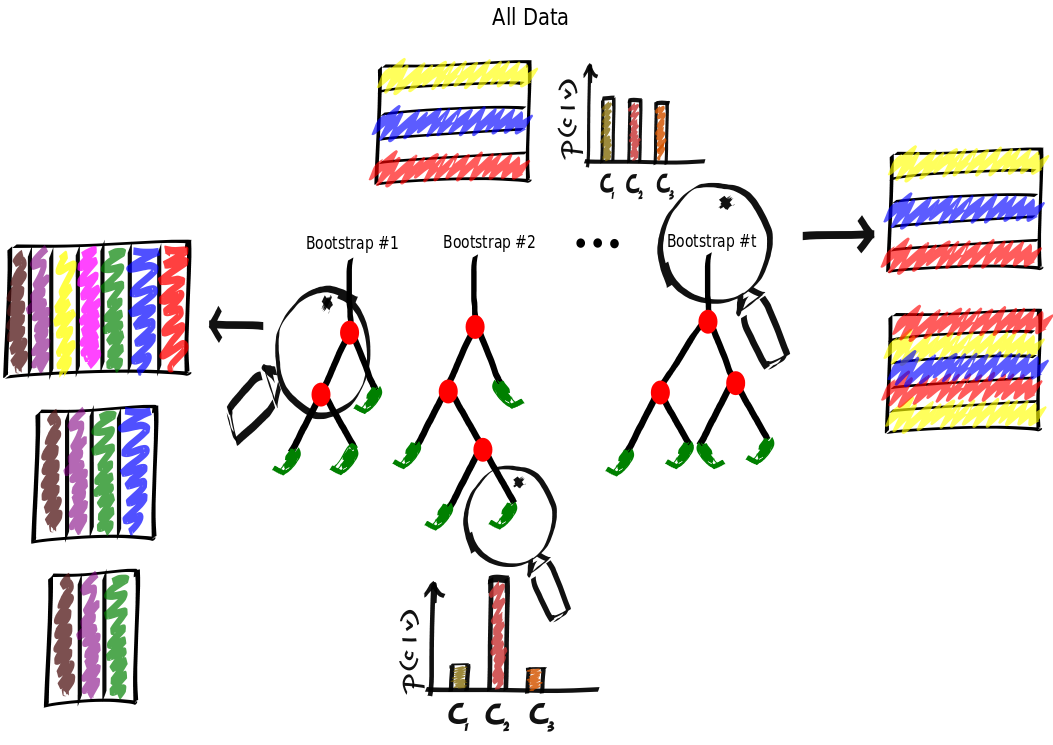
\includegraphics[width = 0.9\textwidth, height = 0.15\textheight]{images/framework/RF_train.png}
            		\end{column}
            		\begin{column}{.44\textwidth}
            		\centering{Testing}\\
            			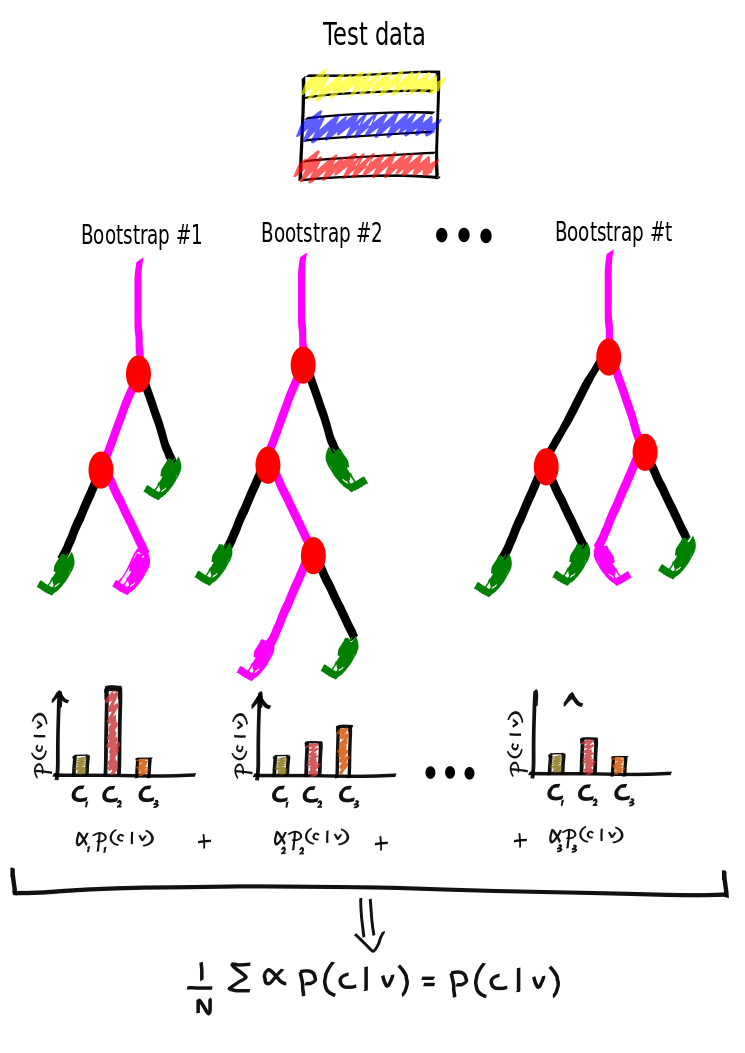
\includegraphics[width = 0.9\textwidth, height = 0.15\textheight]{images/framework/RF_test.png}
            		\end{column}
            \end{columns}
            \item[]
            	\item \textbf{\color{orounam} Weighted combination ensemble}
            \end{itemize}
            \end{block}          
            \vfill
         
          }
        \end{minipage}
      \end{beamercolorbox}
    \end{column}
    %----------------------------------------------------------%
    %             		SECOND COLUMN 						  %
	%----------------------------------------------------------%
	\begin{column}{.49\textwidth}
	\begin{beamercolorbox}[center,wd=\textwidth]{postercolumn}
        \begin{minipage}[T]{.95\textwidth}  % tweaks the width, makes a new \textwidth
          \parbox[t][\columnheight]{\textwidth}{ % must be some better way to set the the height, width and textwidth simultaneously
            % Since all columns are the same length, it is all nice and tidy.  You have to get the height empirically
            \begin{block}{Experiment}
            	 \begin{itemize}
            		\item \textbf{\color{orounam} $PH^{2}$ Dataset}
            		\begin{itemize}
            		 \item First public dermoscopic dataset
            		 \item Acquired at \textit{Dermatology Service of Hospital Pedro Hispano, Matosinhos, Pourtugal}
            		 \item 200 lesions, 40 melanoma, 80 benign and 80 dysplastic lesions 
            		 \item Our subset contains 39 melanoma , 78 benign and 76 dysplastic lesions. Seven lesions are removed due to artefacts such as hair occlusions.
            		\end{itemize}
            		\item \textbf{\color{orounam} Validation}
            		\begin{itemize}
            		 \item Oversampling in order to deal with unbalanced data 
            		 \item Oversampling in \textbf{data space} - generating synthetic melanoma images by deforming the original images
            		 \item First approach: random deformation using Gaussian grid (RDGM) - $N(5,5)$, $R = 80^{\circ}$
            		 \item Second approach: barrel deformation (BD) - barrel distortion , $R = 145^{\circ}$
            		 \item[]
            		 \item[]
            		 \begin{columns}
            		 	\begin{column}{.33\textwidth}
            		 	 	\centering{
            		 		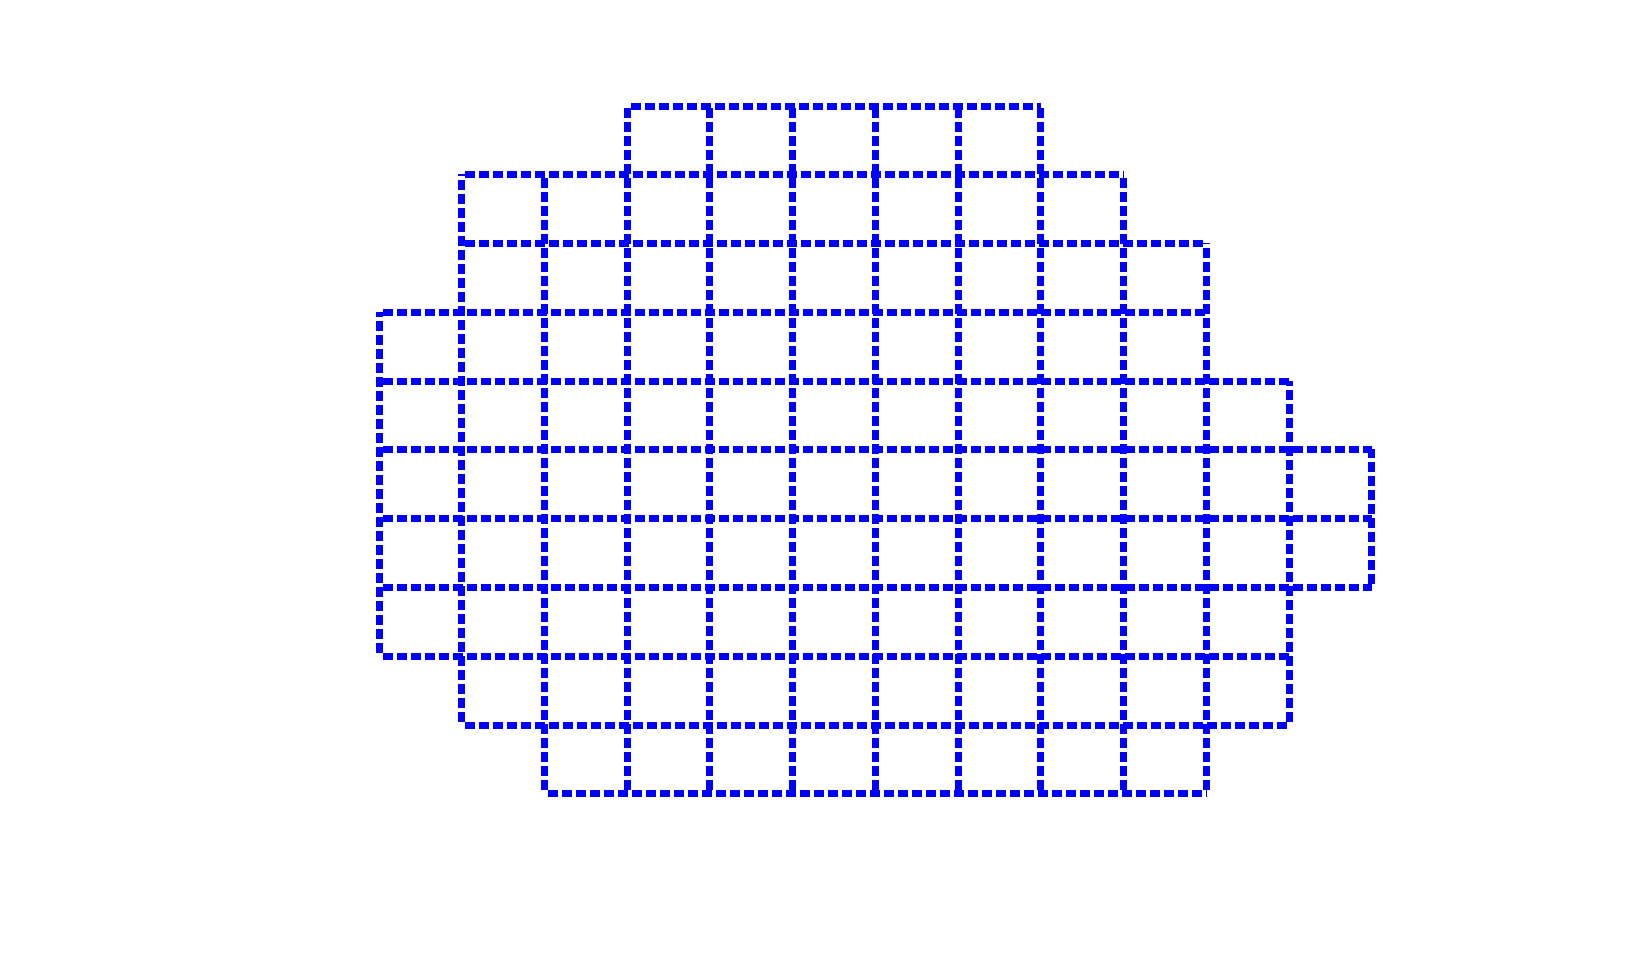
\includegraphics[width=0.8\textwidth]{images/framework/OG.png}}\\
            		 		\centering{Original grid}
            		 	\end{column}
            		 	\begin{column}{.33\textwidth}
            		 	\centering{
            		 		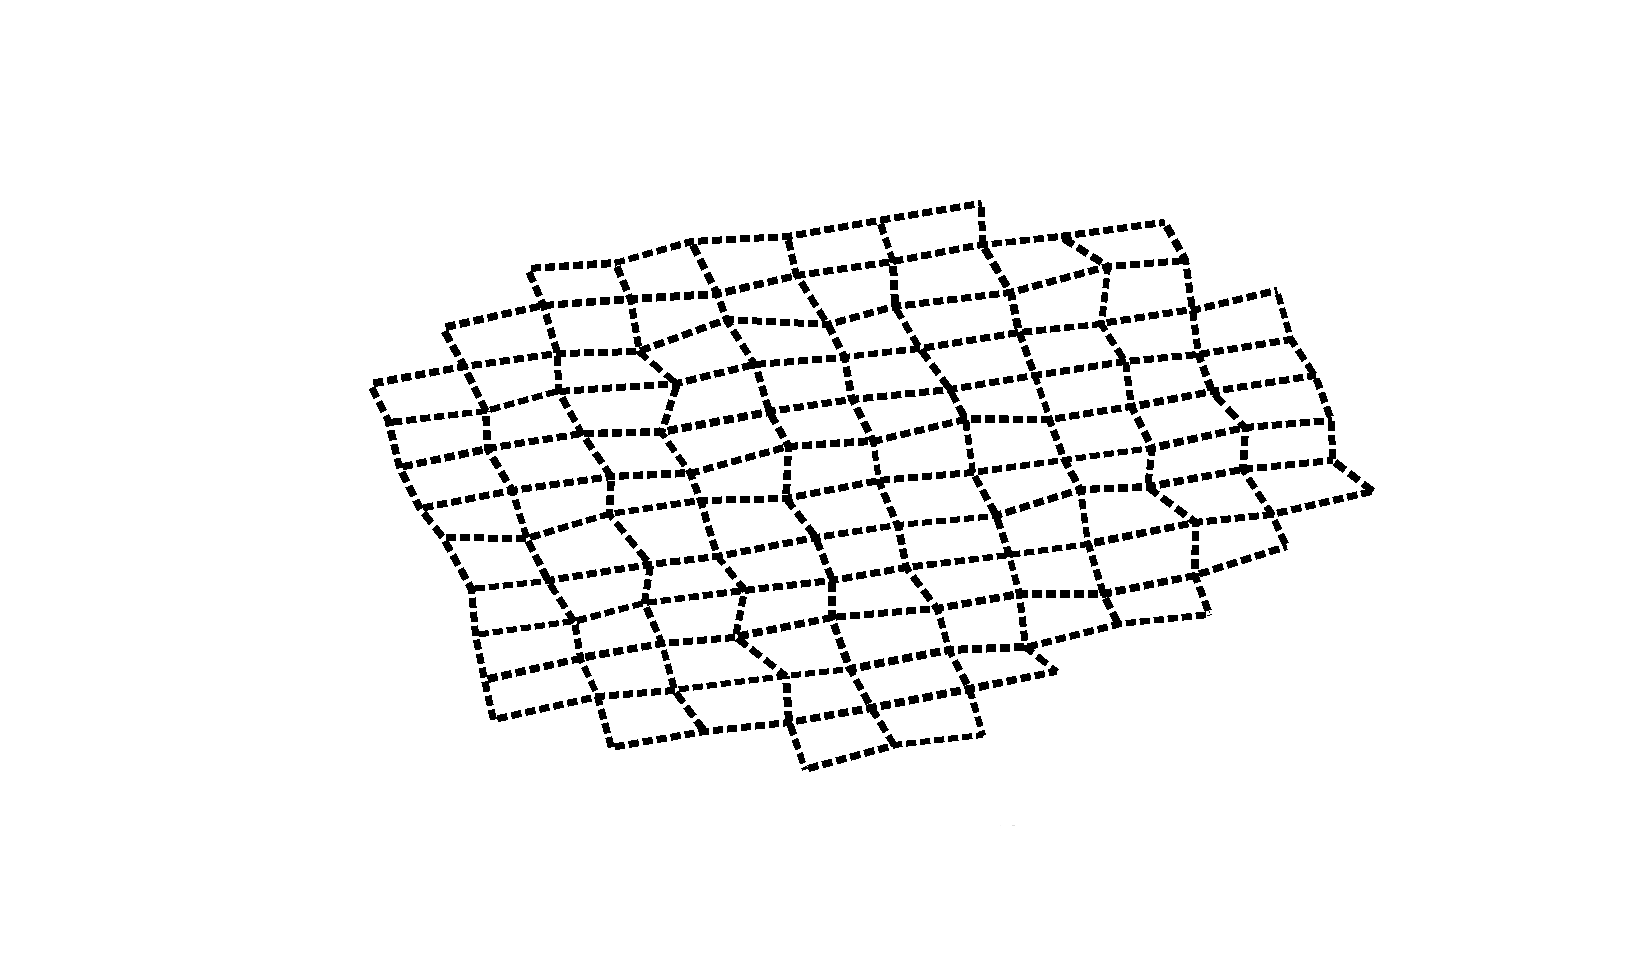
\includegraphics[width=0.8\textwidth]{images/framework/GG3_80.png}}\\
            		 		\centering{RDGM deformation}
            		 	\end{column}
            		 	\begin{column}{.33\textwidth}
            				\centering{
            		 		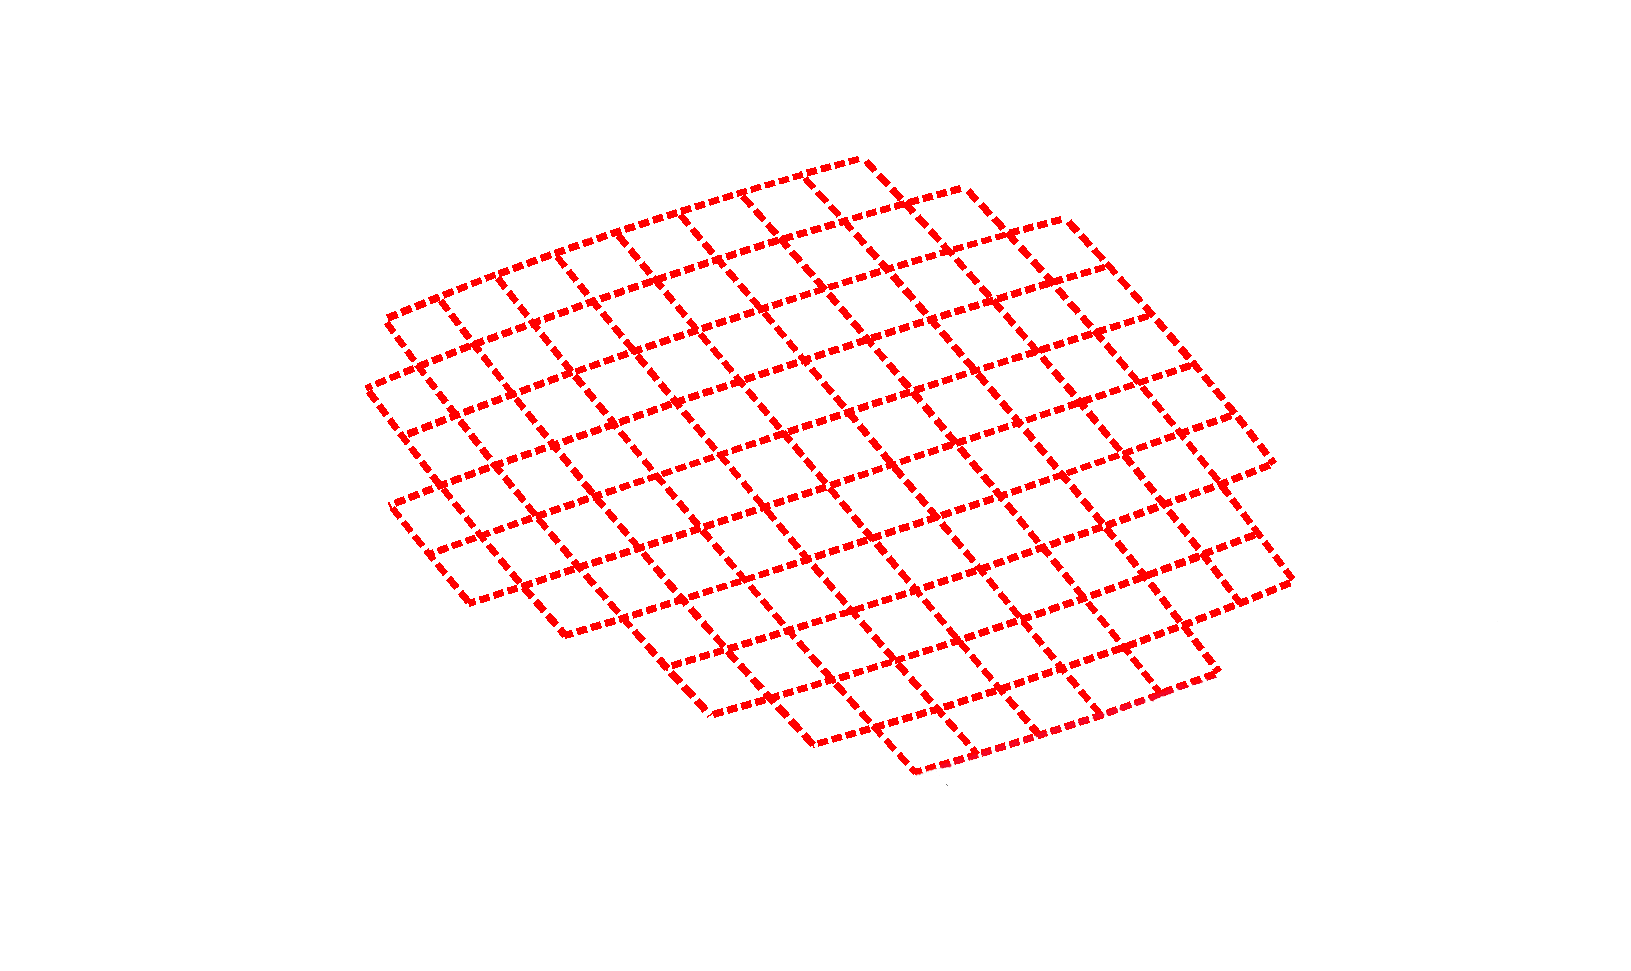
\includegraphics[width=0.8\textwidth]{images/framework/BG3_145.png}}\\
            		 		\centering{BD deformation}
            		 	\end{column}
				\end{columns}
				\item One-vs-all classification
				\end{itemize}
            		
             \end{itemize}
            \end{block}
            \vfill
            \begin{block}{Results}
            \begin{itemize}
            	 \item \textbf{\color{orounam} Individual features}
            	 \item[]        
              \begin{columns}
            	 	\begin{column}{.47\textwidth}
            	 		\centering{
            	 		      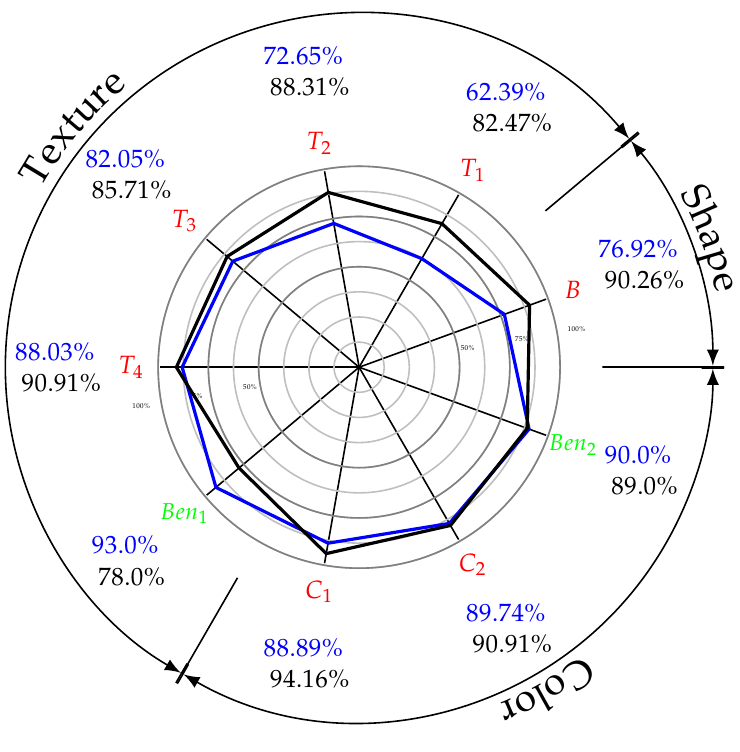
\includegraphics[width=0.6\textwidth]{images/framework/RF_res_indi.png}}\\
            	 		\centering{RF ensemble}
            	 	\end{column}
            	 	\begin{column}{.47\textwidth}
            	 		\centering{
            	 	   	      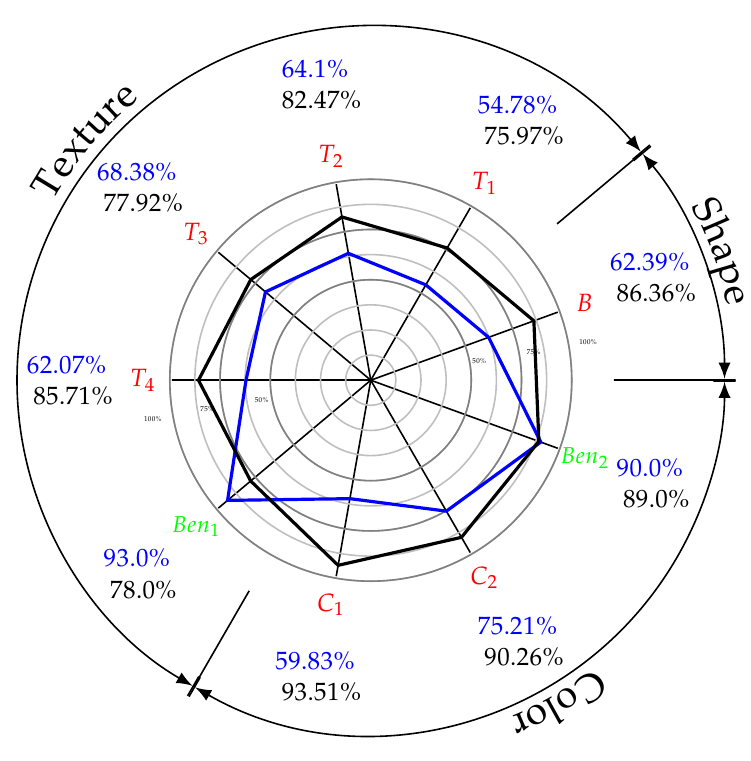
\includegraphics[width=0.6\textwidth]{images/framework/WC_res_indi.png}}\\
            	 	   	\centering{Weighted ensemble}     	 		
            	 	\end{column}
            	 \end{columns}
            	  \item \textbf{\color{orounam} Combination of features}
            	 \item []
            	 \begin{columns}
            	 	\begin{column}{.47\textwidth}
            	 		\centering{
            	 		      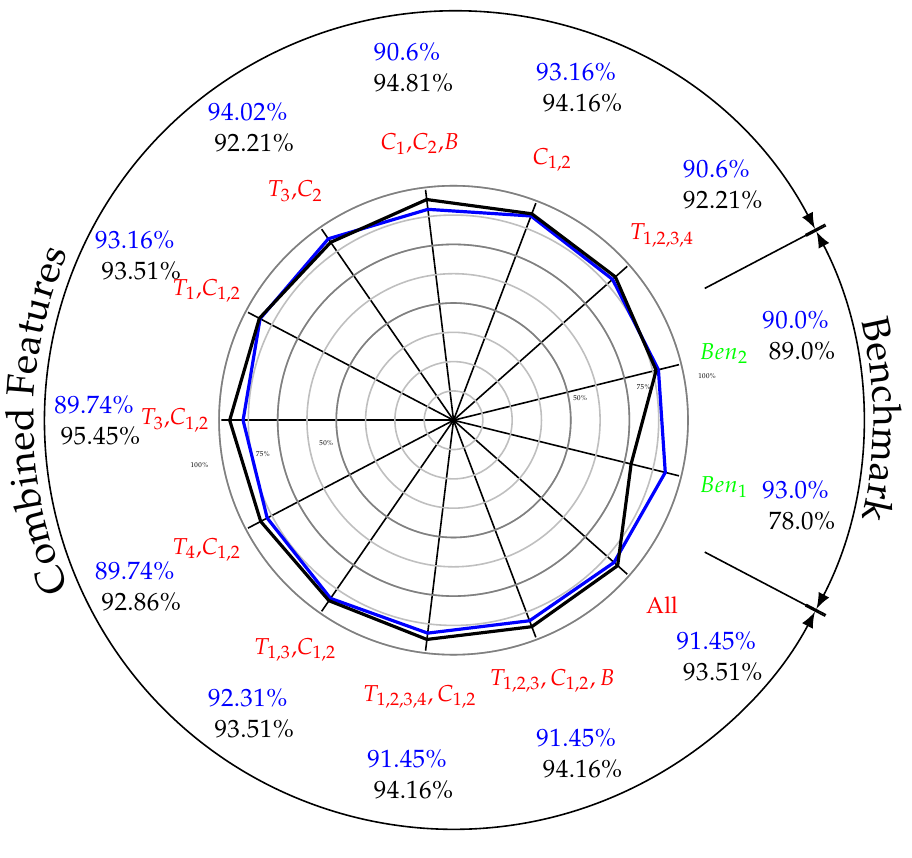
\includegraphics[width=0.8\textwidth]{images/framework/RF_res_com.png}}\\
            	 		      \centering{RF ensemble}
            	 	\end{column}
            	 	\begin{column}{.47\textwidth}
            	 		\centering{
            	 	   	      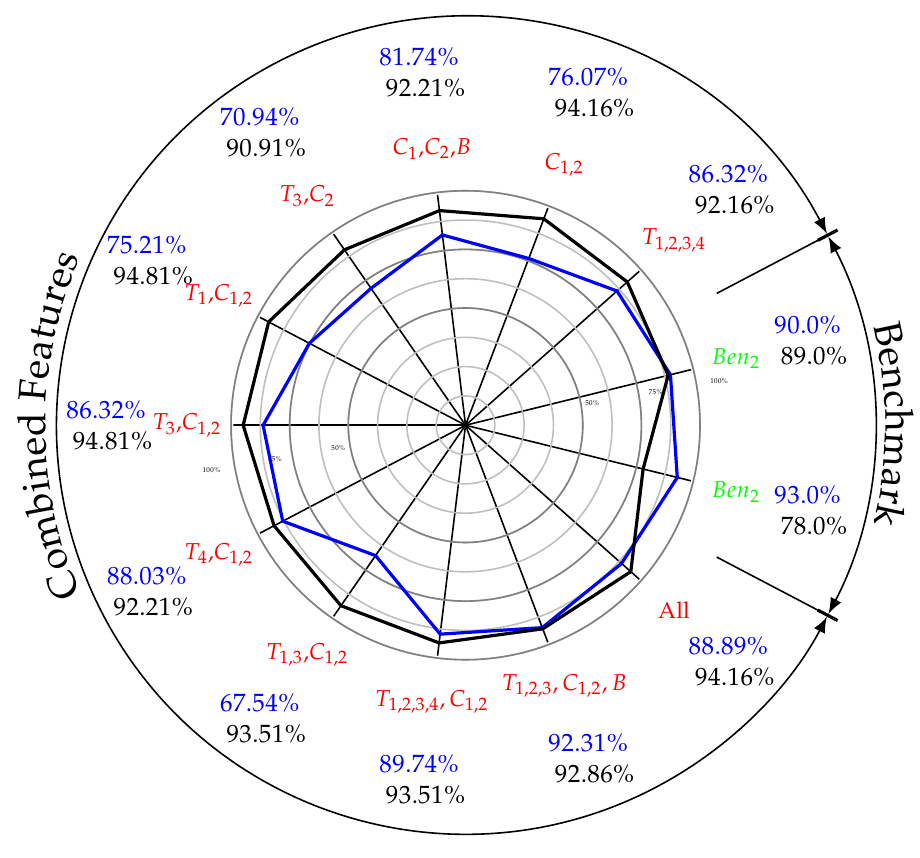
\includegraphics[width=0.8\textwidth]{images/framework/WC_res_com.png}} \\  
            	 	   	      \centering{Weighted combination ensemble}         	 		
            	 	\end{column}
            	 \end{columns}
            	 \item[] The features, sensitivity and specificity are presented in {\color{red} red}, {\color{blue}blue} and black, respectively. The {\color{green}$Ben_{1}$} and {\color{green}$Ben_{2}$} represent the benchmark results, obtained by \cite{barata2013two}. with color and texture features respectively. 
            \end{itemize}
            \end{block}
            \vfill
            \begin{block}{Conclusion}
            \begin{itemize}
            	 \item RF ensemble outperforms the single learners 
            	 \item The obtained results by RF ensemble and combination of several features outperform the benchmark results without over-fitting
            	 \item Texture features such as Histogram of Oriented Gradients and Gabor filters and the new Opponent color angle prove to be effective for classification of melanoma lesions in comparison to previously color and shape features
            \end{itemize}
            
            \end{block}
            \vfill
            \begin{block}{References}
              \bibliography{refs2}
 			  \bibliographystyle{apalike}
            \end{block}
            \vfill
            }
        \end{minipage}
    \end{beamercolorbox}    
	\end{column}
    % ---------------------------------------------------------%
    % end the column
  \end{columns}
  \vskip1ex

  %\tiny\hfill\textcolor{ta2gray}{Created with \LaTeX \texttt{beamerposter}  \url{http://www-i6.informatik.rwth-aachen.de/~dreuw/latexbeamerposter.php}}
  \tiny\hfill{Created with \LaTeX \texttt{beamerposter}  \url{http://www-i6.informatik.rwth-aachen.de/~dreuw/latexbeamerposter.php} \hskip1em}
\end{frame}

\end{document}


%%%%%%%%%%%%%%%%%%%%%%%%%%%%%%%%%%%%%%%%%%%%%%%%%%%%%%%%%%%%%%%%%%%%%%%%%%%%%%%%%%%%%%%%%%%%%%%%%%%%
%%% Local Variables: 
%%% mode: latex
%%% TeX-PDF-mode: t
%%% End:



%            		\subfloat[Grid of original melanoma lesion]{
%					\includegraphics[width=0.30\textwidth]{images/framework/OG_G.png}}\
%					\subfloat[ \nth{1} deformed grid (RDGM) ]{
%					\includegraphics[width=0.30\textwidth]{images/framework/GG_80_G.png}}\
%					\subfloat[\nth{2} deformed grid (BD)]{
%					\includegraphics[width=0.30\textwidth]{images/framework/BG_145_G.png}}
%					\caption{Deformation approaches used for melanoma lesions}